%!TEX TS-program = xelatex
\documentclass[]{friggeri-cv}
\usepackage{afterpage}
\usepackage{hyperref}
\usepackage{color}
\usepackage{xcolor}
\hypersetup{
    pdftitle={},
    pdfauthor={},
    pdfsubject={},
    pdfkeywords={},
    colorlinks=false,       % no lik border color
   allbordercolors=white    % white border color for all
}
\addbibresource{bibliography.bib}
\RequirePackage{xcolor}
\definecolor{pblue}{HTML}{0395DE}

\begin{document}
\header{Tyler }{ Lyle}
      {Software Engineer}
      
% Fake text to add separator      
\fcolorbox{white}{gray}{\parbox{\dimexpr\textwidth-2\fboxsep-2\fboxrule}{%
.....
}}

% In the aside, each new line forces a line break
\begin{aside}
  \section{Address}
    2115 New Road
    Waterford, PA 16441
    ~
  \section{Telephone}
    +1 (814) 464 3068
    ~
  \section{Mail}
    \href{mailto:}{\textbf{jobsearch\_lylet@}\\yahoo.com}
    ~
  \section{Web \& Git}
    \href{https://tyler-lyle.netlify.com/}{tyler-lyle.netlify.com}
    \href{https://bitbucket.org/tylerlyle}{bitbucket.org/\textbf{tylerlyle}}
    \href{https://github.com/lylet-AC}{github.com/\textbf{lylet-AC}}
    ~
  \section{Programming}
    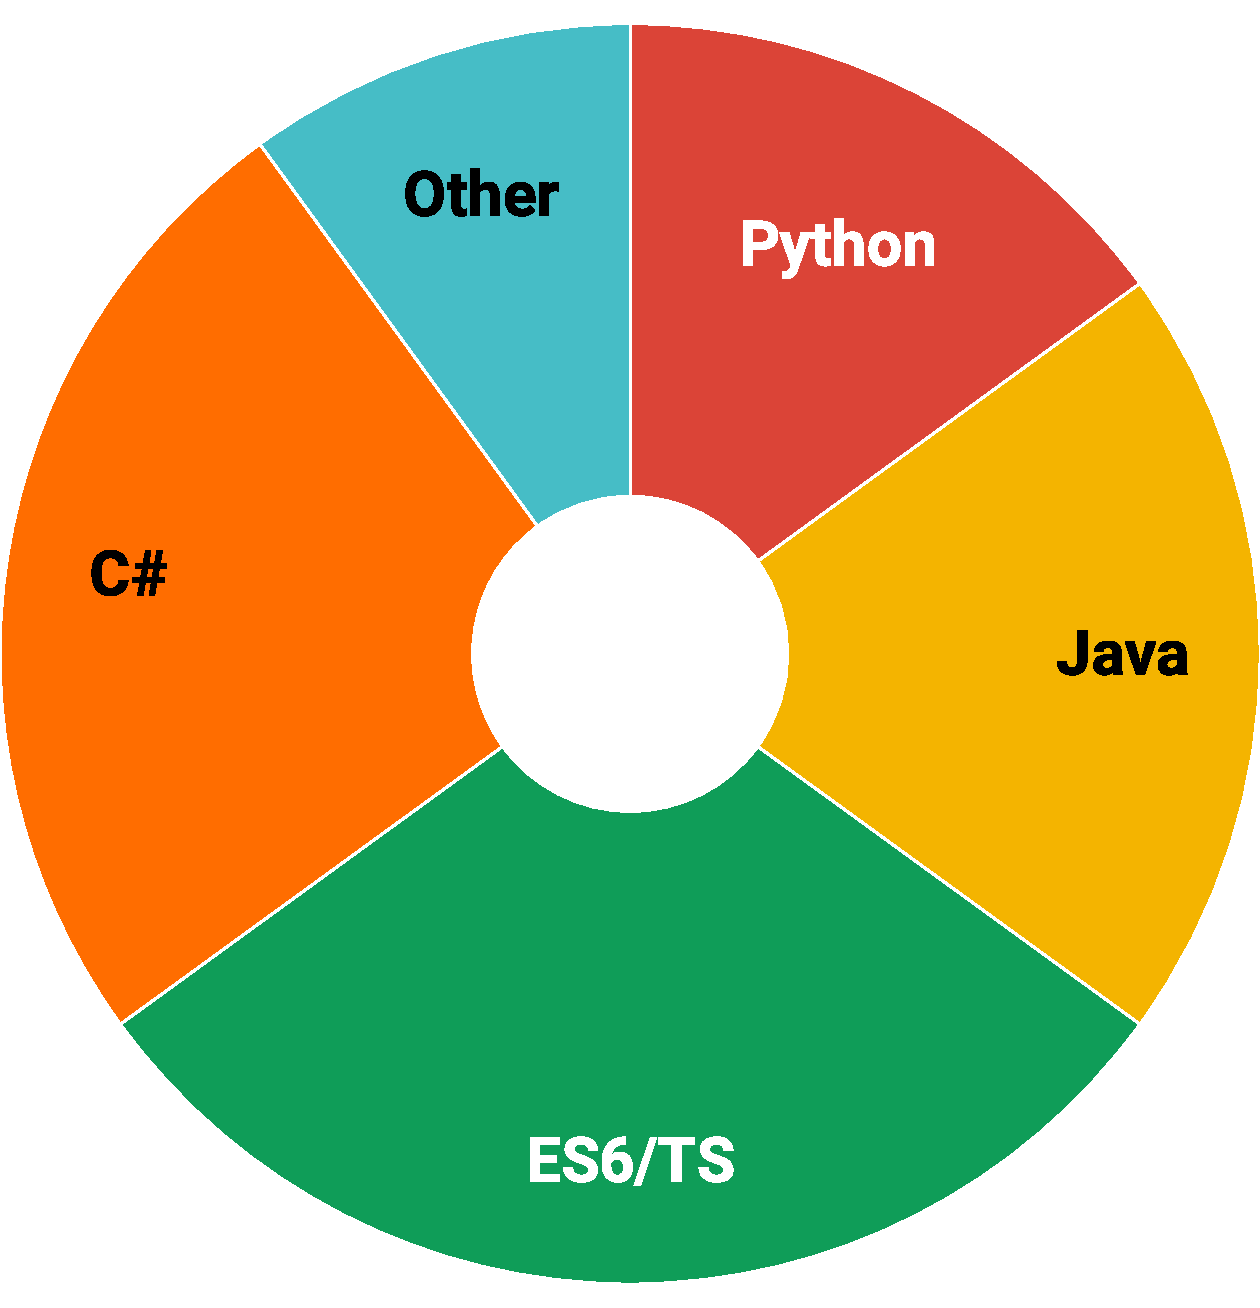
\includegraphics[scale=0.18]{img/pvl.pdf}
    ~
  \section{OS Preference}
    \textbf{GNU/Linux}
\includegraphics[scale=0.40]{img/5stars.png}
    \textbf{MacOS}
\includegraphics[scale=0.40]{img/3stars.png}
    \textbf{Windows}
\includegraphics[scale=0.40]{img/4stars.png}
    ~
  \section{Personal Skills}
    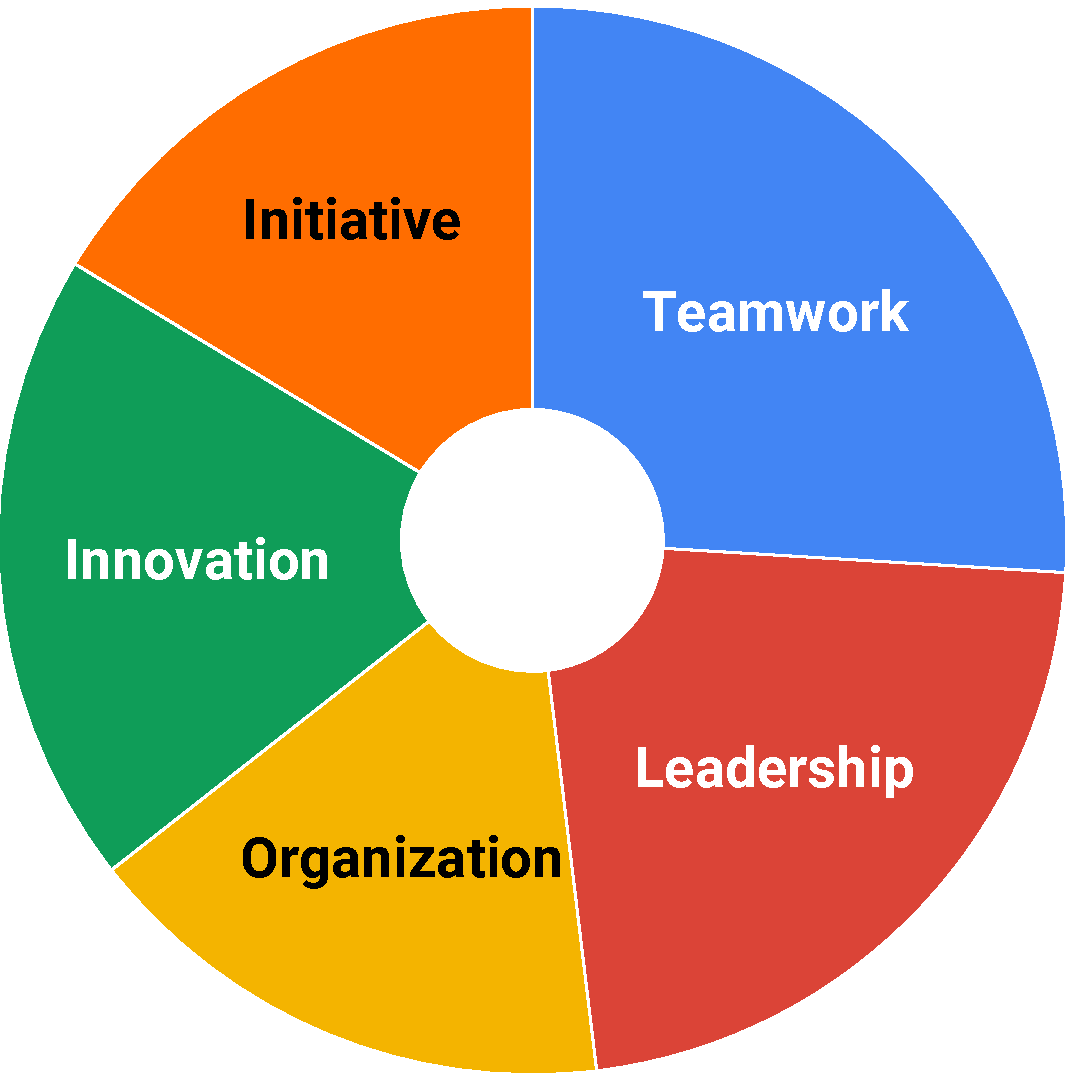
\includegraphics[scale=0.2]{img/skills.pdf}
    ~
\end{aside}

\section{About Me}
\begin{entrylist}
	\entry
	{}
	{Computer Enthusiast}
	{First Generation College Student}
	{Ever since I was young, I was fascinated with computers. As a low income family, my father could not afford a new computer to support this interest.  Therefore, my first computer was a laptop constructed from other recycled and broken laptops.  Given our low income status, I could also not afford to purchase a Windows XP license. As such, I spent most of my time from 8 years old using machines operating various Linux distributions.\\
	
	From here, my father and I spent countless hours learning web development and I.T. together, with my first programming language being JavaScript.  Even after he decided to exit the field in 2017, my love for computers did not dwindle.  I am currently graduating Allegheny College in 2019 with a degree in Computer Science, and a concentration in Software Development.  To me, the field of C.S. is not just a career, it is a passion.

}
\end{entrylist}

\section{Experience}
\begin{entrylist}
  \entry
    {6/17 - Now}
    {POS Operator}
    {Kohl's Department Store}
    {Guarantee customer satisfaction, solicit Kohl's Charge store cards, cash out customers, evening cash management.\\}
  \entry
    {6/13 - 2/18}
    {Shift Supervisor \& Closing Manager}
    {The Wendy's Company}
    {Ensure that food meets safety and quality standards, conduct interviews, train crew members, evening cash management, nightly inventory audits, establish goals.\\}
\end{entrylist}

\section{Education}
\begin{entrylist}
  \entry
    {2015 - 2019}
    {Bachelor's Degree in Computer Science}
    {Allegheny College}
    {Software Engineering.\\
    Main subjects: Software Engineering, Artificial Intelligence, Distributed Cloud Systems, Web Development.\\
    \emph{Title of the Thesis: "Pynesthesia: Creating Tile Maps with Color"      .}\\
    \emph{Relators: Prof. Janyl Jumadinova, Prof. Aravind Mohan.}\\}

  \entry
    {2011 - 2015}
    {High School Diploma}
    {McDowell High School}
    {Secondary School.\\
    Main subjects: Computer Science, Game Design, AutoCAD, Engineering.\\}

  \entry
	{2013 - 2014}
	{No Certification}
	{Erie County Technical School}
	{Vocational Tech School.\\
	Main subjects: Computer Science, Electrical Engineering.\\}
\end{entrylist}

\begin{flushleft}
\emph{April 21st, 2019}
\end{flushleft}
\begin{flushright}
\emph{Tyler Lyle}
\end{flushright}

\end{document}
